\chapter{Imaging and Tracking Payload Unit}
\label{chap:itpu}

The \ac{ITPU} is the scientific payload of the airship. The purpose of the \ac{ITPU} is to take aerial images from different positions, acquire accurate position and attitude data and use that combined information to create aerial image maps. This subsystem is in general independent of the airship's control system, but it uses the airship's \ac{EPS}. It would however be possible in an extended version to also incorporate a controlling interface and to connect the motor \ac{ESC}s to the computer of the \ac{ITPU}. 
\\
\\
 The subsystem is split up into the following parts:
\begin{itemize}
\item Attitude determination: use an advanced data fusion method to facilitate \ac{GPS}, gyroscope, accelerometer and magnetometer information and to extract accurate position and attitude information together with reasonable error estimates.
\item Imaging system: provide images with a megapixel resolution webcam in regular time-steps in the order of a second. The image data is saved on a \ac{SD} memory card together with the attitude information for off-line processing.
\item Communication system: transmit attitude data and telemetry to a ground station.
\item Image processing software: image matching and evaluation on a standard computer after payload
recovery.
\end{itemize}

\pagebreak

\section{Functional and Technical Requirements}

The functional requirements of the \ac{ITPU} are listed below.

\begin{itemize}
\item Measure absolute and accurate position and pointing angles
\item Take images in regular time-steps and save them together with attitude data
\item Receive and execute basic telecommands such as image capture start/stop
\item Send basic telemetry data (e.g. position) to a ground station
\item Combine single image captures into a large area map
\end{itemize}

\noindent
The technical requirements are listed in Table \ref{tab:technical}.

\begin{table}[H]
\centering
\caption{Technical requirements}
\label{tab:technical}
\begin{minipage}{\textwidth}
\begin{tabular}{p{0.4\textwidth}p{0.15\textwidth}p{0.45\textwidth}}
\hline
\textbf{Parameter} & \textbf{Value} & \textbf{Remarks}\\ \hline
Operation altitude & $< 500\,m$\footnote{The \ac{U-SPACE} requirements are less stringent, but the \ac{ITPU} might be used at these altitudes in later applications} & Open air\\
Input voltage & $5\,V$ & Un-regulated\\
Maximum power consumption  & $2.5\,W$ & -\\
Image storage capacity & $>\,1000$ & 1 Mega-pixel resolution\\
\hline
\end{tabular}\par
\vspace{-0.75\skip\footins}
\renewcommand{\footnoterule}{}
\end{minipage}
\vspace{-1.0em}
\end{table}

\section{Electronic Components}

\subsection{Board Computer}

To read out the sensors, communicate with the ground station and save images from the camera, an embedded system which provides all necessary interfaces and sufficient computing power to handle comparably large data streams from the camera is required. The BeagleBone \cite{website:beaglebone, BeagleBone:SRM} was selected, but only the BeagleBoard \cite{website:beagleboard} was delivered, which is a related predecessor that lacks some features.
\\
\\
The BeagleBoard is a microcontroller board running a TI OMAP3530 ARM Cortex-A8 \ac{SoC}. It provides 256~MB RAM and several high and low level interfaces. The main interfaces used for the \ac{U-SPACE} project are \ac{$I^2C$} and \ac{UART} for communication with the sensors (gyroscope, magnetometer, accelerometer) and the \ac{GPS}-receiver and radio-transmitter module (E-TAG). The high level interface to connect the camera is the \ac{USB}-host adapter. The operating system with the control program as well as the image files are stored onto an 8~GB class 10 \ac{SD} card. The required supply voltage for the BeagleBoard is 5~V. The voltage of the pins on the extension header is 1.8~V.

\subsection{Sensors}

To determine the position and attitude of the airship the LSM303DLM \cite{LSM303:datasheet} combined magnetometer and accelerometer and the ITG-3200 triple-axis gyroscope \cite{ITG-3200:datasheet} from Sparkfun are used. Both sensors have been used by the team members during an earlier project. The sensors communicate via an \ac{$I^2C$} interface with the main board at 3.3~V. To receive \ac{GPS} information an E-TAG device developed by Esrange is
used. It is connected via a serial line interface with the main board. It also provides a transmitter module for communication with the ground station which however, will not be used for U-SPACE.

\subsection{Camera}

As high-quality embedded industrial cameras are very highly priced, a consumer webcam with a resolution of several megapixels will be connected to the \ac{USB}-port of the main board. It is planned to acquire a camera which is supported by the Linux operating system running on the main board.

%\subsection{Attitude Determination System}

\FloatBarrier
\section{Software Environment}

The BeagleBoard is equipped with an 8~GB micro-\ac{SD} card. A Debian-based Linux operating system is installed onto the card providing the environment, libraries and drivers for the program to run. As compared to the BeagleBone the
BeagleBoard lacks pull-up resistors on its \ac{$I^2C$} interface which produces problems with the Linux kernel. Also, the standard kernel for this board came without the possibility to enable the \ac{$I^2C$} controller. Therefore a custom version of the Linux kernel was compiled for the BeagleBoard in order to activate the \ac{$I^2C$} device on the extension header. 
\\
\\
The OnBoard program is divided into five threads. One thread is responsible for getting the newest sensor data from the accelerometer, magnetometer and gyroscope through the \ac{$I^2C$} interface and fusing them to achieve accurate position and attitude representations. This thread is running at a relatively high frequency (>50 Hz, but the final frequency has not yet been defined).  A second thread is polling for new \ac{GPS} data from the E-TAG via a serial line. As the \ac{GPS}-chip only updates the positional data about once per second this thread can run at a much lower frequency. A third thread is responsible for controlling the camera and if active, it will take a picture every second and save it to the \ac{SD}-card. The two final threads handle the sending of telemetry data to and the receiving of basic commands from the ground station, respectively.

\noindent
Due to a lack of time a standard kernel is used which is not hard real-time capable. Nevertheless it still has the possibility of using pre-emptive scheduling which should give a high enough accuracy. It should be noted that in future
developments it could be beneficial to use a real-time Linux kernel.

\FloatBarrier
\section{Image Processing}

The provided sensory and computational system (the \ac{U-SPACE} \ac{ITPU}) is meant to be a cradle for image processing experiments that simulate low earth orbit conditions. Given the meta-information available from the images, several basic scenarios can be assumed:

\begin{itemize}
\item Aerial map creation (optionally automatic)
\item 3D reconstruction of large areas
\item Object tracking
\item Visual attitude determination
\end{itemize}

\noindent
The basic design of each possibility and its scientific potential are briefly discussed in this section.

\subsection{Camera Calibration}

A simple and low-cost camera is being used, but, nevertheless, the system has to be calibrated and projection distortion has to be compensated. Since it is assumed that pictures are taken at larger distances than the camera was designed for, this distortion compensation is crucial for a proper output quality. The camera parameters are modelled assuming a simple pin-hole camera. Pictures of a well known pattern with easily detectable lines or points on lines are taken. Taking various pictures of a tilted chess board pattern allows to stably detect corners of the pattern. The corners are lying on a straight line (under a rotation-translation transformation). Using this information the so-called intrinsic camera parameters can be calculated. As the straight lines of points will appear to be curved on the pictures, a transformation can be computed to straighten up these lines and thus compensate for the lens distortion. There might be a need for future extrinsic camera calibration as well. This is important especially for 3D and automated applications where a coordinate frame is required.

\subsection{Preprocessing}
\label{sec:preprocessing}

A crucial step for quality assurance is the first preprocessing and data homologization step. The input picture needs to be as clear and dynamically stable as possible as well as distortion free. There might be more steps involved, but the most important ones are lens distortion compensation, contrast and brightness stabilization and blur removal. Lens distortion compensation is a compensation of the lens's radial character and comes as the calibration result. Contrast and brightness might be adjusted globally to avoid saturated or noisy pictures. It is assumed that the aerial carrier is moving and without suitable light conditions the image can get blurry. To compensate for this blur a motion blur
removal filter has to be deployed. Assuming linear and constant motion a Wiener filter can be implemented. The motion
can be estimated from the sensors or through image analysis. 

\subsection{Aerial Map Creation}

Creating an aerial map or stitching partial views into a single picture is a basic space-related operation. The implemented approach consists of the following steps:

\begin{enumerate}
\item Preprocessing
\item Feature detection
\item Feature rejection
\item Transformation estimation
\item Transformation
\item Image merging
\end{enumerate}

\noindent
Preprocessing was described in section \ref{sec:preprocessing}. Feature detection is then the next step. As there
are many feature detectors there is a possibility to evaluate the performance of different feature detectors on different
climates or terrain types. It was decided to implement three feature extraction methods to start with. These methods are the well-known SIFT keypoints, Kanade Lucas Tomasi (KLT) tracker based features and AGAST - a machine-generated corner detector developed at DLR for robust 3D reconstruction.
\\
\\
Feature rejection then filters wrong data or data irrelevant to the transformation that is under investigation. It can also filter bad features, that are not persistent in the pictures long enough. Based on the geometry of the detected features and sensor information affine transformation parameters can be estimated at the minimum. All of these methods should provide enough control points so that it would be possible to estimate an even higher polynomial transformation to ease the image stitching at the edges.
\\
\\
After carrying out the transformation the pictures can be merged with small overlapping regions around the edges, followed by a smooth transition from picture to picture. This process can be handled by the processing unit on-the-fly such that the \ac{ITPU} is able to provide a ready-made result.

\subsection{3D Reconstruction of Large Objects}

Another potential application is robust 3D object reconstruction. Having multiple arbitrary views of one large object (for example a castle), it is possible to find regions that are invariant to an affine transformation. With these regions the position and parameters of the camera can be calculated as well as a transformation of the key points. This solution is based on the MSER algorithm and implemented in OpenCV.

\subsection{Object Tracking}

In case the \ac{ITPU} has control over the steering of the airship a real-time object tracking system could be implemented. Tracking is a modified recognition problem which focuses on real-time performance. A continuous target movement is assumed, which allows to incorporate filtering and movement prediction methods such as a Kalman filter. 

\subsection{Visual Attitude Determination}

Another important usage possibility is attitude determination. From the relative transformation in-between images a relative six degrees of freedom pose change can be estimated. Having samples of absolute reference this pose can be cleaned of incremental errors and a long time solution can be tested. Such an algorithm could even be used for planetary and interplanetary localization.

\FloatBarrier
\section{Attitude Determination System}

The \ac{ADS} measures and estimates the position and pointing direction of the payload system. This function is crucial for the further use of recorded images, as it provides the reference system and the relative alignment of the recorded images towards each other. In order to produce high-accuracy attitude estimates and to compensate for disadvantages of certain sensor types such as drift and noise, a variety of sensors is used and their data is fused to provide complete attitude information. An overview of the \ac{ADS} is shown in Figure \ref{fig:ADS_overview}.
\vspace{1.0em}

\begin{figure}
\centering
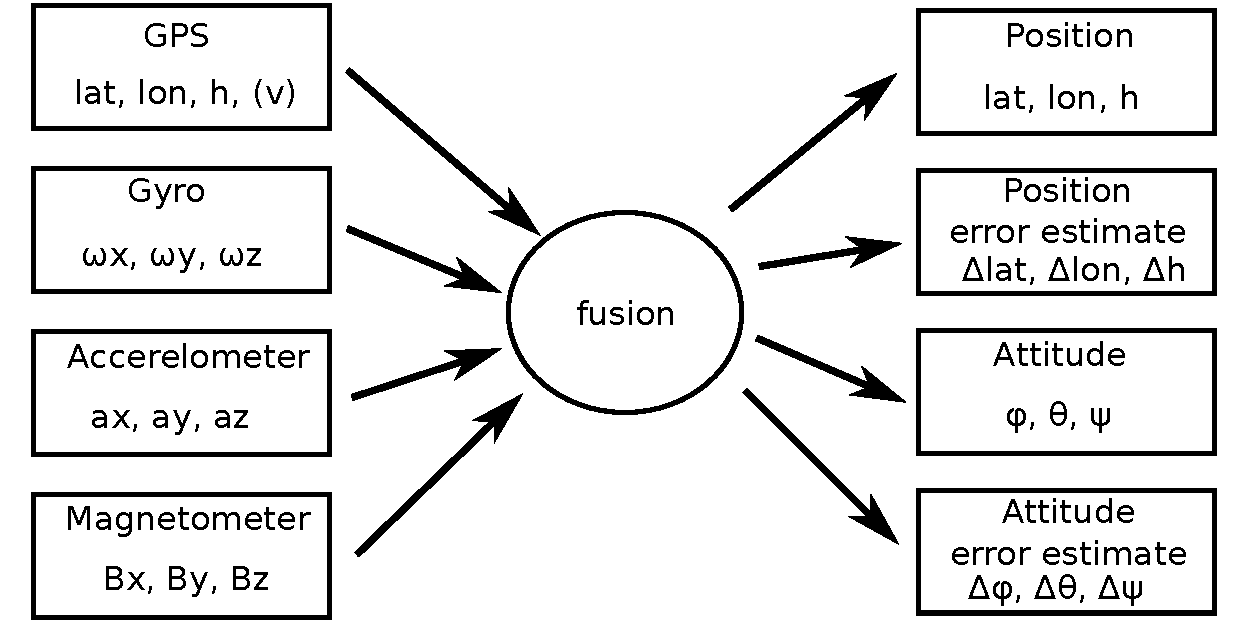
\includegraphics[width=0.73\textwidth]{figures/ADS_diagram.pdf}
\caption{\acl{ADS} overview}
\label{fig:ADS_overview}
\end{figure}

\noindent
As can be seen in Figure \ref{fig:ADS_overview}, the sensors to be used are:

\begin{itemize}
\item \ac{GPS} receiver: provides absolute position values, but has much high-frequency noise
\item Gyroscope: provides accurate relative pointing directions, but experiences drift
\item Accelerometer: provides absolute pointing relative to the horizon (gravity) and linear acceleration
\item Magnetometer: provides absolute pointing relative to the earth's magnetic field
\end{itemize}

%\FloatBarrier
\subsection{Development Status}

The \ac{ADS} has not only been developed on the final hardware (BeagleBoard). To continue the development during the semester break a recently released Raspberry Pi minicomputer \cite{website:raspberry} has been privately purchased, with properties very similar to the BeagleBoard. It also runs a derivative of the Debian operating system. A board has been created to attach a complete set of sensors to the system. These sensors are a gyroscope (ITG-3200 from Sparkfun), a magnetometer/accelerometer (LSM303 from Sparkfun) and a \ac{GPS} receiver(Etag). All sensors are pluggable and the complete system is shown in Figure \ref{fig:raspberry-sensors-top}(A Venus 6 \ac{GPS} Module ST22 from SkyTraq has been used in the shown figure). The bottom side of the board including the wiring cables is shown in Figure \ref{fig:raspberry-sensors-open}. This testing system does not yet contain a camera, but it will be added in the future. In this configuration the entire unit consumes 3 W of power and weighs 71 g (broken down into 30 g for the sensors and shield and 41 g for the computer).

\begin{figure}[h!]
\centering
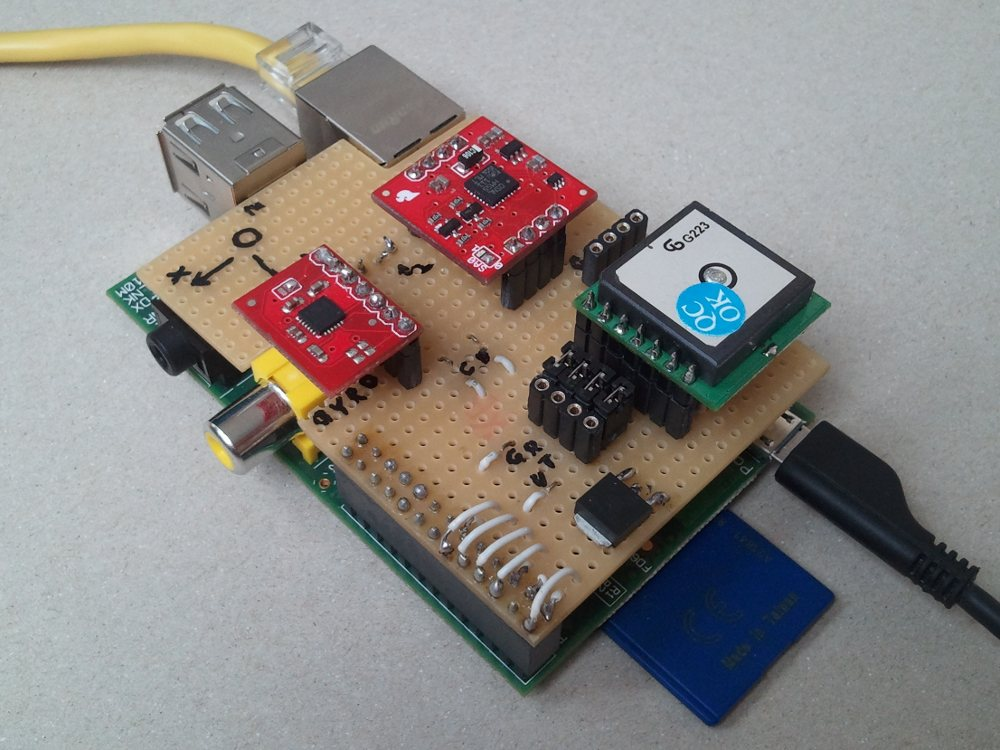
\includegraphics[width=0.8\textwidth]{figures/raspberry-sensors-top.jpg}
\caption[Top view of Raspberry Pi computer with sensor shield]{Top view of Raspberry Pi computer with self-constructed pluggable sensor shield. Mounted on the shield are the gyroscope (red, left), the magnetometer/accelerometer (red, top) and the \ac{GPS} receiver (green, right). Also \ac{$I^2C$} and \ac{UART} 4-pin sockets are visible as well as a small voltage regulator (bottom) that connects the 3.3 V \ac{GPS} module to the 5 V high-current source.}
\label{fig:raspberry-sensors-top}
\end{figure}

\pagebreak

\begin{figure}[h!]
\centering
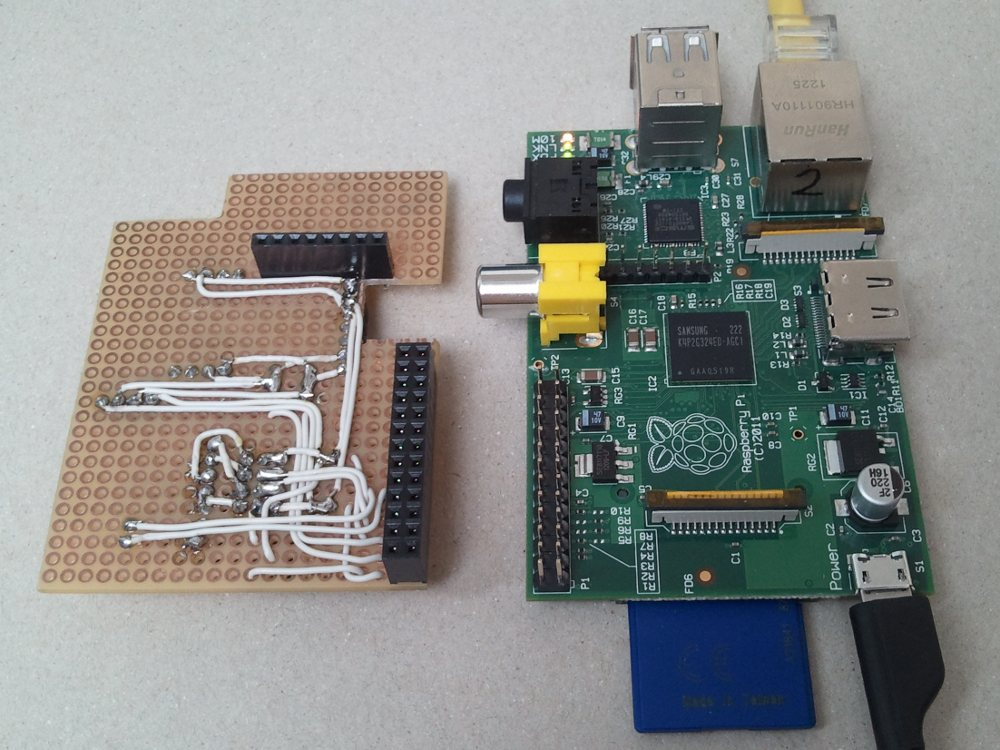
\includegraphics[width=0.8\textwidth]{figures/raspberry-sensors-open.jpg}
\caption[Bottom view of opened-up Raspberry Pi computer with sensor shield]{Bottom view of opened-up Raspberry Pi computer with self-constructed pluggable sensor shield. Wiring from the Raspberry Pi 26-pin P1 header to the individual sensors can be seen on the bottom side of the shield.}
\label{fig:raspberry-sensors-open}
\vspace{-1.0em}
\end{figure}

%% more text until end of august if I [Bastian] find time.

\subsection{Algorithms}

The attitude of the sensing unit could in principle be determined by simply integrating the gyroscope rates from an initial alignment. This measurement however will degrade with time because of significant low-frequency drifts, sensor offsets and measurement inaccuracies. To solve the problem more robustly a combination of 3D gyroscope, a magnetometer and an accelerometer is used. They are fused with a C++ program that runs on the board computer. The main technique used is the \ac{EKF} which offers a near-optimal attitude estimation with a fixed memory usage. Attitudes are represented as quaternions, which is an elegant and \ac{CPU}-effective solution.
\\
\\
Offset filtering for the magnetometer and accelerometer is performed independently. An \ac{EKF} has been set up that estimates the $x$- $y$- and $z$-offset and the total radius along with each new measurement. The measurements are readily available at system start-up without calibration, but the accuracy will only improve as soon as measurements from different attitudes are available. The \ac{EKF} also accounts for slow offset drifts and similar effects.
%% more text until end of august if I [Bastian] find time.
\\
\\
An estimation of the gyroscope offsets and rate scaling is performed with a combination of accelerometer and magnetometer absolute attitude estimations and the gyroscope-integrated attitude. This results in a gyroscope error value at each measurement step that is used by the Kalman algorithm to estimate the system parameters and to calculate a best-estimate attitude.
%% more text until end of august if I [Bastian] find time.
\\
\\
Finally the position is determined independently from the \ac{GPS} receiver, which is much simpler than fusing position values from the inertial measurement of the previously described sensors with the absolute \ac{GPS} position. This approach was chosen due to the tight time constraints of the project. However, in a continuation of the project it is desirable to test the fusion algorithm described in \cite[chap. 6.4]{book:stochastic}.
%% more text until end of august if I [Bastian] find time.

\FloatBarrier
\section{Electrical Circuits}

As compared to the BeagleBone the voltage of the delivered BeagleBoard at the pins of the extension header is only between 0~V and 1.8~V. However, the expected voltage at the supply and at the \ac{$I^2C$} interface for the sensors is 3.3~V. Thus additionally to the external pull-up resistors on the \ac{$I^2C$} interface also voltage level converters have to be used for the BeagleBoard.